\documentclass{standalone}
\usepackage{tikz}
\usetikzlibrary{patterns, positioning}


\begin{document}
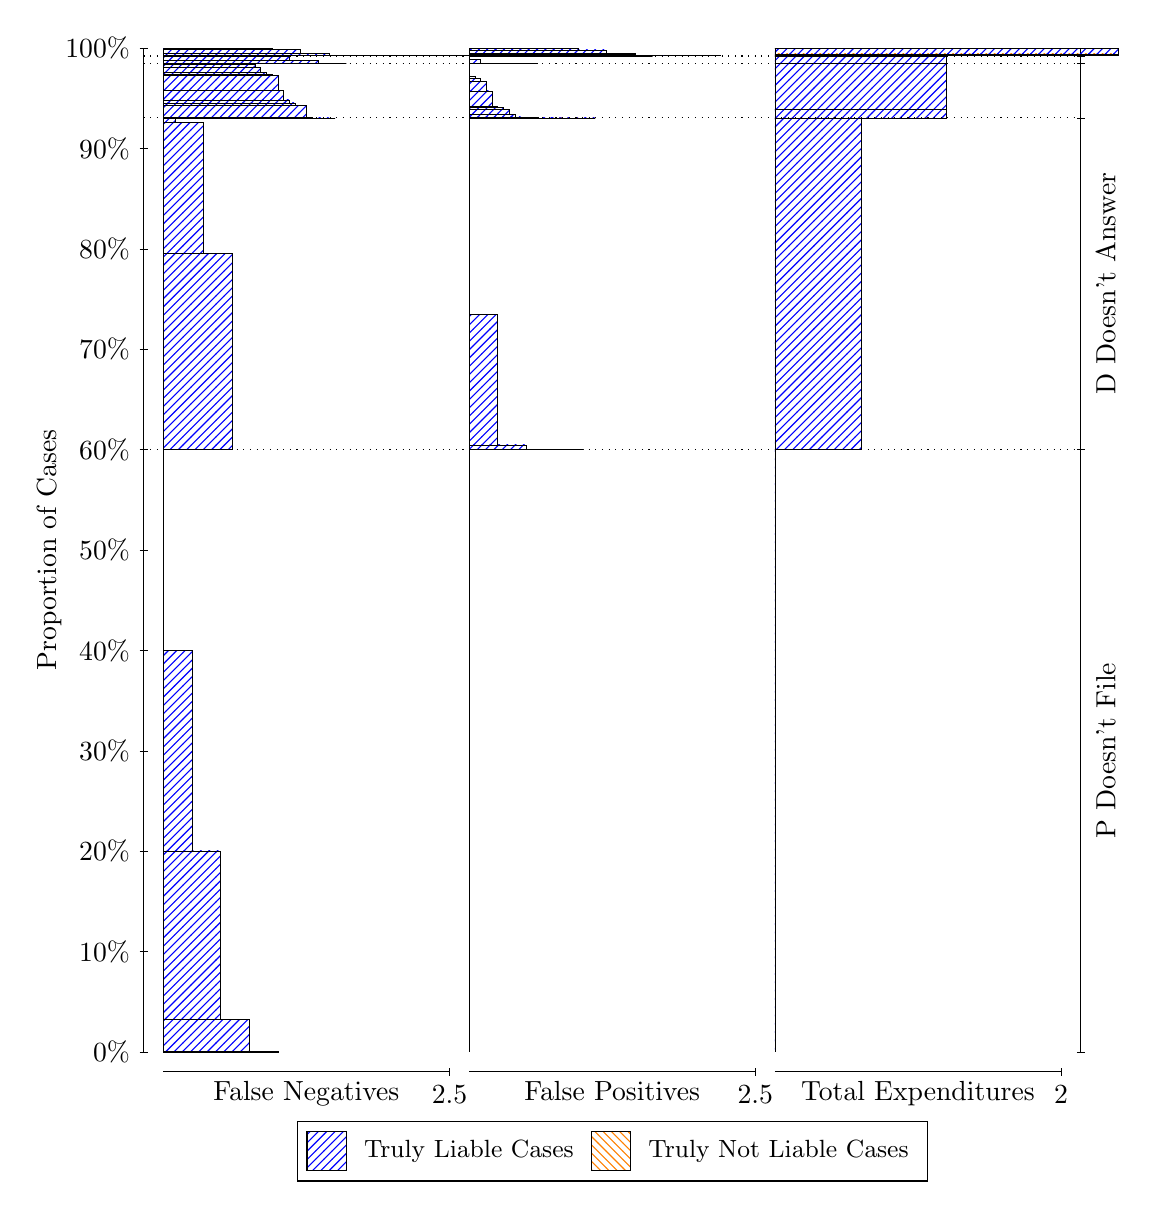
\begin{tikzpicture}
\draw[black, very thin] (1.5,1.75) -- (1.5,14.5);
\node[rotate=90, text=black, anchor=center] at (0.3, 8.125) {Proportion of Cases};
\draw[black, very thin] (1.45,1.75) -- (1.55,1.75);
\node[text=black, anchor=east] at (1.45, 1.75) {0\%};
\draw[black, very thin] (1.45,3.025) -- (1.55,3.025);
\node[text=black, anchor=east] at (1.45, 3.025) {10\%};
\draw[black, very thin] (1.45,4.3) -- (1.55,4.3);
\node[text=black, anchor=east] at (1.45, 4.3) {20\%};
\draw[black, very thin] (1.45,5.575) -- (1.55,5.575);
\node[text=black, anchor=east] at (1.45, 5.575) {30\%};
\draw[black, very thin] (1.45,6.85) -- (1.55,6.85);
\node[text=black, anchor=east] at (1.45, 6.85) {40\%};
\draw[black, very thin] (1.45,8.125) -- (1.55,8.125);
\node[text=black, anchor=east] at (1.45, 8.125) {50\%};
\draw[black, very thin] (1.45,9.4) -- (1.55,9.4);
\node[text=black, anchor=east] at (1.45, 9.4) {60\%};
\draw[black, very thin] (1.45,10.675) -- (1.55,10.675);
\node[text=black, anchor=east] at (1.45, 10.675) {70\%};
\draw[black, very thin] (1.45,11.95) -- (1.55,11.95);
\node[text=black, anchor=east] at (1.45, 11.95) {80\%};
\draw[black, very thin] (1.45,13.225) -- (1.55,13.225);
\node[text=black, anchor=east] at (1.45, 13.225) {90\%};
\draw[black, very thin] (1.45,14.5) -- (1.55,14.5);
\node[text=black, anchor=east] at (1.45, 14.5) {100\%};

\draw[black, very thin] (13.4,1.75) -- (13.4,14.5);
\draw[black, very thin] (13.35,1.75) -- (13.45,1.75);
\node[anchor=west] at (13.35, 1.75) {};
\draw[black, very thin] (13.35,9.4013) -- (13.45,9.4013);
\node[anchor=west] at (13.35, 9.4013) {};
\draw[black, very thin] (13.35,13.613) -- (13.45,13.613);
\node[anchor=west] at (13.35, 13.613) {};
\draw[black, very thin] (13.35,14.301) -- (13.45,14.301);
\node[anchor=west] at (13.35, 14.301) {};
\draw[black, very thin] (13.35,14.393) -- (13.45,14.393);
\node[anchor=west] at (13.35, 14.393) {};
\draw[black, very thin] (13.35,14.407) -- (13.45,14.407);
\node[anchor=west] at (13.35, 14.407) {};
\draw[black, very thin] (13.35,14.5) -- (13.45,14.5);
\node[anchor=west] at (13.35, 14.5) {};

\draw[black, very thin, pattern color=blue, pattern=north east lines] (1.75,1.75) rectangle (3.2033,1.7541);
\draw[black, very thin, pattern color=blue, pattern=north east lines] (1.75,1.7541) rectangle (2.84,2.1592);
\draw[black, very thin, pattern color=blue, pattern=north east lines] (1.75,2.1592) rectangle (2.4767,4.3047);
\draw[black, very thin, pattern color=blue, pattern=north east lines] (1.75,4.3047) rectangle (2.1133,6.8513);
\draw[black, very thin, pattern color=orange, pattern=north west lines] (1.75,6.8513) rectangle (1.75,6.8513);
\draw[black, very thin, pattern color=blue, pattern=north east lines] (1.75,6.8513) rectangle (1.75,9.4013);
\draw[black, very thin, pattern color=blue, pattern=north east lines] (1.75,9.4013) rectangle (2.622,11.896);
\draw[black, very thin, pattern color=blue, pattern=north east lines] (1.75,11.896) rectangle (2.2587,13.555);
\draw[black, very thin, pattern color=blue, pattern=north east lines] (1.75,13.555) rectangle (1.8953,13.613);
\draw[black, very thin, pattern color=orange, pattern=north west lines] (1.75,13.613) rectangle (1.75,13.613);
\draw[black, very thin, pattern color=blue, pattern=north east lines] (1.75,13.613) rectangle (1.75,13.613);
\draw[black, very thin, pattern color=blue, pattern=north east lines] (1.75,13.613) rectangle (3.93,13.613);
\draw[black, very thin, pattern color=blue, pattern=north east lines] (1.75,13.613) rectangle (3.7847,13.613);
\draw[black, very thin, pattern color=blue, pattern=north east lines] (1.75,13.613) rectangle (3.6393,13.62);
\draw[black, very thin, pattern color=blue, pattern=north east lines] (1.75,13.62) rectangle (3.5667,13.771);
\draw[black, very thin, pattern color=blue, pattern=north east lines] (1.75,13.771) rectangle (3.494,13.772);
\draw[black, very thin, pattern color=blue, pattern=north east lines] (1.75,13.772) rectangle (3.4213,13.802);
\draw[black, very thin, pattern color=blue, pattern=north east lines] (1.75,13.802) rectangle (3.3487,13.842);
\draw[black, very thin, pattern color=blue, pattern=north east lines] (1.75,13.842) rectangle (3.276,13.958);
\draw[black, very thin, pattern color=blue, pattern=north east lines] (1.75,13.958) rectangle (3.2033,14.154);
\draw[black, very thin, pattern color=blue, pattern=north east lines] (1.75,14.154) rectangle (3.1307,14.163);
\draw[black, very thin, pattern color=blue, pattern=north east lines] (1.75,14.163) rectangle (3.058,14.193);
\draw[black, very thin, pattern color=blue, pattern=north east lines] (1.75,14.193) rectangle (2.9853,14.256);
\draw[black, very thin, pattern color=blue, pattern=north east lines] (1.75,14.256) rectangle (2.9127,14.289);
\draw[black, very thin, pattern color=blue, pattern=north east lines] (1.75,14.289) rectangle (2.84,14.291);
\draw[black, very thin, pattern color=blue, pattern=north east lines] (1.75,14.291) rectangle (2.7673,14.296);
\draw[black, very thin, pattern color=blue, pattern=north east lines] (1.75,14.296) rectangle (2.6947,14.296);
\draw[black, very thin, pattern color=blue, pattern=north east lines] (1.75,14.296) rectangle (2.622,14.301);
\draw[black, very thin, pattern color=blue, pattern=north east lines] (1.75,14.301) rectangle (2.5493,14.301);
\draw[black, very thin, pattern color=blue, pattern=north east lines] (1.75,14.301) rectangle (2.4767,14.301);
\draw[black, very thin, pattern color=blue, pattern=north east lines] (1.75,14.301) rectangle (2.404,14.301);
\draw[black, very thin, pattern color=blue, pattern=north east lines] (1.75,14.301) rectangle (2.3313,14.301);
\draw[black, very thin, pattern color=blue, pattern=north east lines] (1.75,14.301) rectangle (2.2587,14.301);
\draw[black, very thin, pattern color=blue, pattern=north east lines] (1.75,14.301) rectangle (2.186,14.301);
\draw[black, very thin, pattern color=blue, pattern=north east lines] (1.75,14.301) rectangle (2.0407,14.301);
\draw[black, very thin, pattern color=blue, pattern=north east lines] (1.75,14.301) rectangle (1.8953,14.301);
\draw[black, very thin, pattern color=orange, pattern=north west lines] (1.75,14.301) rectangle (1.75,14.301);
\draw[black, very thin, pattern color=blue, pattern=north east lines] (1.75,14.301) rectangle (4.0753,14.301);
\draw[black, very thin, pattern color=blue, pattern=north east lines] (1.75,14.301) rectangle (3.712,14.342);
\draw[black, very thin, pattern color=blue, pattern=north east lines] (1.75,14.342) rectangle (3.3487,14.392);
\draw[black, very thin, pattern color=blue, pattern=north east lines] (1.75,14.392) rectangle (2.9853,14.393);
\draw[black, very thin, pattern color=blue, pattern=north east lines] (1.75,14.393) rectangle (2.622,14.393);
\draw[black, very thin, pattern color=orange, pattern=north west lines] (1.75,14.393) rectangle (1.75,14.393);
\draw[black, very thin, pattern color=blue, pattern=north east lines] (1.75,14.393) rectangle (2.622,14.394);
\draw[black, very thin, pattern color=blue, pattern=north east lines] (1.75,14.394) rectangle (2.2587,14.403);
\draw[black, very thin, pattern color=blue, pattern=north east lines] (1.75,14.403) rectangle (1.8953,14.407);
\draw[black, very thin, pattern color=orange, pattern=north west lines] (1.75,14.407) rectangle (1.75,14.407);
\draw[black, very thin, pattern color=blue, pattern=north east lines] (1.75,14.407) rectangle (1.75,14.407);
\draw[black, very thin, pattern color=blue, pattern=north east lines] (1.75,14.407) rectangle (8.4353,14.407);
\draw[black, very thin, pattern color=blue, pattern=north east lines] (1.75,14.407) rectangle (8.072,14.407);
\draw[black, very thin, pattern color=blue, pattern=north east lines] (1.75,14.407) rectangle (7.7087,14.407);
\draw[black, very thin, pattern color=blue, pattern=north east lines] (1.75,14.407) rectangle (7.3453,14.408);
\draw[black, very thin, pattern color=blue, pattern=north east lines] (1.75,14.408) rectangle (6.982,14.408);
\draw[black, very thin, pattern color=blue, pattern=north east lines] (1.75,14.408) rectangle (6.6187,14.408);
\draw[black, very thin, pattern color=blue, pattern=north east lines] (1.75,14.408) rectangle (6.2553,14.408);
\draw[black, very thin, pattern color=blue, pattern=north east lines] (1.75,14.408) rectangle (4.584,14.408);
\draw[black, very thin, pattern color=blue, pattern=north east lines] (1.75,14.408) rectangle (4.2207,14.409);
\draw[black, very thin, pattern color=blue, pattern=north east lines] (1.75,14.409) rectangle (3.8573,14.431);
\draw[black, very thin, pattern color=blue, pattern=north east lines] (1.75,14.431) rectangle (3.494,14.478);
\draw[black, very thin, pattern color=blue, pattern=north east lines] (1.75,14.478) rectangle (3.1307,14.499);
\draw[black, very thin, pattern color=blue, pattern=north east lines] (1.75,14.499) rectangle (2.7673,14.5);
\draw[black, very thin, pattern color=blue, pattern=north east lines] (1.75,14.5) rectangle (2.404,14.5);
\draw[black, very thin, pattern color=blue, pattern=north east lines] (1.75,14.5) rectangle (2.0407,14.5);
\draw[black, very thin, pattern color=orange, pattern=north west lines] (1.75,14.5) rectangle (1.75,14.5);
\draw[black, very thin, pattern color=orange, pattern=north west lines] (5.6333,1.75) rectangle (5.6333,1.75);
\draw[black, very thin, pattern color=blue, pattern=north east lines] (5.6333,1.75) rectangle (5.6333,9.4013);
\draw[black, very thin, pattern color=orange, pattern=north west lines] (5.6333,9.4013) rectangle (7.0867,9.4013);
\draw[black, very thin, pattern color=blue, pattern=north east lines] (5.6333,9.4013) rectangle (7.0867,9.4013);
\draw[black, very thin, pattern color=blue, pattern=north east lines] (5.6333,9.4013) rectangle (6.7233,9.4013);
\draw[black, very thin, pattern color=blue, pattern=north east lines] (5.6333,9.4013) rectangle (6.36,9.4592);
\draw[black, very thin, pattern color=blue, pattern=north east lines] (5.6333,9.4592) rectangle (5.9967,11.118);
\draw[black, very thin, pattern color=blue, pattern=north east lines] (5.6333,11.118) rectangle (5.6333,13.613);
\draw[black, very thin, pattern color=orange, pattern=north west lines] (5.6333,13.613) rectangle (7.232,13.613);
\draw[black, very thin, pattern color=blue, pattern=north east lines] (5.6333,13.613) rectangle (7.232,13.613);
\draw[black, very thin, pattern color=orange, pattern=north west lines] (5.6333,13.613) rectangle (7.0867,13.613);
\draw[black, very thin, pattern color=blue, pattern=north east lines] (5.6333,13.613) rectangle (7.0867,13.613);
\draw[black, very thin, pattern color=orange, pattern=north west lines] (5.6333,13.613) rectangle (6.9413,13.613);
\draw[black, very thin, pattern color=blue, pattern=north east lines] (5.6333,13.613) rectangle (6.9413,13.613);
\draw[black, very thin, pattern color=blue, pattern=north east lines] (5.6333,13.613) rectangle (6.8687,13.613);
\draw[black, very thin, pattern color=orange, pattern=north west lines] (5.6333,13.613) rectangle (6.796,13.613);
\draw[black, very thin, pattern color=blue, pattern=north east lines] (5.6333,13.613) rectangle (6.796,13.613);
\draw[black, very thin, pattern color=blue, pattern=north east lines] (5.6333,13.613) rectangle (6.7233,13.613);
\draw[black, very thin, pattern color=orange, pattern=north west lines] (5.6333,13.613) rectangle (6.6507,13.613);
\draw[black, very thin, pattern color=blue, pattern=north east lines] (5.6333,13.613) rectangle (6.6507,13.613);
\draw[black, very thin, pattern color=blue, pattern=north east lines] (5.6333,13.613) rectangle (6.578,13.613);
\draw[black, very thin, pattern color=blue, pattern=north east lines] (5.6333,13.613) rectangle (6.5053,13.618);
\draw[black, very thin, pattern color=blue, pattern=north east lines] (5.6333,13.618) rectangle (6.4327,13.618);
\draw[black, very thin, pattern color=blue, pattern=north east lines] (5.6333,13.618) rectangle (6.36,13.623);
\draw[black, very thin, pattern color=blue, pattern=north east lines] (5.6333,13.623) rectangle (6.2873,13.625);
\draw[black, very thin, pattern color=blue, pattern=north east lines] (5.6333,13.625) rectangle (6.2147,13.658);
\draw[black, very thin, pattern color=blue, pattern=north east lines] (5.6333,13.658) rectangle (6.142,13.721);
\draw[black, very thin, pattern color=blue, pattern=north east lines] (5.6333,13.721) rectangle (6.0693,13.751);
\draw[black, very thin, pattern color=blue, pattern=north east lines] (5.6333,13.751) rectangle (5.9967,13.76);
\draw[black, very thin, pattern color=blue, pattern=north east lines] (5.6333,13.76) rectangle (5.924,13.956);
\draw[black, very thin, pattern color=blue, pattern=north east lines] (5.6333,13.956) rectangle (5.8513,14.072);
\draw[black, very thin, pattern color=blue, pattern=north east lines] (5.6333,14.072) rectangle (5.7787,14.112);
\draw[black, very thin, pattern color=blue, pattern=north east lines] (5.6333,14.112) rectangle (5.706,14.142);
\draw[black, very thin, pattern color=blue, pattern=north east lines] (5.6333,14.142) rectangle (5.6333,14.301);
\draw[black, very thin, pattern color=orange, pattern=north west lines] (5.6333,14.301) rectangle (6.5053,14.301);
\draw[black, very thin, pattern color=blue, pattern=north east lines] (5.6333,14.301) rectangle (6.5053,14.301);
\draw[black, very thin, pattern color=blue, pattern=north east lines] (5.6333,14.301) rectangle (6.142,14.302);
\draw[black, very thin, pattern color=blue, pattern=north east lines] (5.6333,14.302) rectangle (5.7787,14.353);
\draw[black, very thin, pattern color=blue, pattern=north east lines] (5.6333,14.353) rectangle (5.6333,14.393);
\draw[black, very thin, pattern color=orange, pattern=north west lines] (5.6333,14.393) rectangle (7.9587,14.393);
\draw[black, very thin, pattern color=blue, pattern=north east lines] (5.6333,14.393) rectangle (7.9587,14.393);
\draw[black, very thin, pattern color=blue, pattern=north east lines] (5.6333,14.393) rectangle (7.5953,14.393);
\draw[black, very thin, pattern color=blue, pattern=north east lines] (5.6333,14.393) rectangle (7.232,14.396);
\draw[black, very thin, pattern color=blue, pattern=north east lines] (5.6333,14.396) rectangle (6.8687,14.406);
\draw[black, very thin, pattern color=blue, pattern=north east lines] (5.6333,14.406) rectangle (6.5053,14.407);
\draw[black, very thin, pattern color=orange, pattern=north west lines] (5.6333,14.407) rectangle (8.8307,14.407);
\draw[black, very thin, pattern color=blue, pattern=north east lines] (5.6333,14.407) rectangle (8.8307,14.407);
\draw[black, very thin, pattern color=blue, pattern=north east lines] (5.6333,14.407) rectangle (8.4673,14.407);
\draw[black, very thin, pattern color=orange, pattern=north west lines] (5.6333,14.407) rectangle (8.4673,14.407);
\draw[black, very thin, pattern color=blue, pattern=north east lines] (5.6333,14.407) rectangle (8.4673,14.407);
\draw[black, very thin, pattern color=blue, pattern=north east lines] (5.6333,14.407) rectangle (8.104,14.407);
\draw[black, very thin, pattern color=orange, pattern=north west lines] (5.6333,14.407) rectangle (8.104,14.407);
\draw[black, very thin, pattern color=blue, pattern=north east lines] (5.6333,14.407) rectangle (8.104,14.407);
\draw[black, very thin, pattern color=blue, pattern=north east lines] (5.6333,14.407) rectangle (7.7407,14.423);
\draw[black, very thin, pattern color=orange, pattern=north west lines] (5.6333,14.423) rectangle (7.7407,14.423);
\draw[black, very thin, pattern color=blue, pattern=north east lines] (5.6333,14.423) rectangle (7.7407,14.428);
\draw[black, very thin, pattern color=blue, pattern=north east lines] (5.6333,14.428) rectangle (7.3773,14.43);
\draw[black, very thin, pattern color=blue, pattern=north east lines] (5.6333,14.43) rectangle (7.3773,14.476);
\draw[black, very thin, pattern color=blue, pattern=north east lines] (5.6333,14.476) rectangle (7.014,14.497);
\draw[black, very thin, pattern color=blue, pattern=north east lines] (5.6333,14.497) rectangle (6.6507,14.499);
\draw[black, very thin, pattern color=blue, pattern=north east lines] (5.6333,14.499) rectangle (6.2873,14.499);
\draw[black, very thin, pattern color=orange, pattern=north west lines] (5.6333,14.499) rectangle (5.6333,14.499);
\draw[black, very thin, pattern color=blue, pattern=north east lines] (5.6333,14.499) rectangle (5.6333,14.5);
\draw[black, very thin, pattern color=orange, pattern=north west lines] (9.5167,1.75) rectangle (9.5167,1.75);
\draw[black, very thin, pattern color=blue, pattern=north east lines] (9.5167,1.75) rectangle (9.5167,9.4013);
\draw[black, very thin, pattern color=orange, pattern=north west lines] (9.5167,9.4013) rectangle (10.607,9.4013);
\draw[black, very thin, pattern color=blue, pattern=north east lines] (9.5167,9.4013) rectangle (10.607,13.613);
\draw[black, very thin, pattern color=orange, pattern=north west lines] (9.5167,13.613) rectangle (11.697,13.613);
\draw[black, very thin, pattern color=blue, pattern=north east lines] (9.5167,13.613) rectangle (11.697,13.72);
\draw[black, very thin, pattern color=orange, pattern=north west lines] (9.5167,13.72) rectangle (11.697,13.72);
\draw[black, very thin, pattern color=blue, pattern=north east lines] (9.5167,13.72) rectangle (11.697,14.301);
\draw[black, very thin, pattern color=orange, pattern=north west lines] (9.5167,14.301) rectangle (11.697,14.301);
\draw[black, very thin, pattern color=blue, pattern=north east lines] (9.5167,14.301) rectangle (11.697,14.393);
\draw[black, very thin, pattern color=orange, pattern=north west lines] (9.5167,14.393) rectangle (11.697,14.393);
\draw[black, very thin, pattern color=blue, pattern=north east lines] (9.5167,14.393) rectangle (11.697,14.407);
\draw[black, very thin, pattern color=orange, pattern=north west lines] (9.5167,14.407) rectangle (13.877,14.407);
\draw[black, very thin, pattern color=blue, pattern=north east lines] (9.5167,14.407) rectangle (13.877,14.425);
\draw[black, very thin, pattern color=orange, pattern=north west lines] (9.5167,14.425) rectangle (13.877,14.425);
\draw[black, very thin, pattern color=blue, pattern=north east lines] (9.5167,14.425) rectangle (13.877,14.499);
\draw[black, very thin, pattern color=orange, pattern=north west lines] (9.5167,14.499) rectangle (13.877,14.499);
\draw[black, very thin, pattern color=blue, pattern=north east lines] (9.5167,14.499) rectangle (13.877,14.5);
\draw[black, dotted] (1.5,9.4013) -- (13.4,9.4013);
\draw[black, dotted] (1.5,13.613) -- (13.4,13.613);
\draw[black, dotted] (1.5,14.301) -- (13.4,14.301);
\draw[black, dotted] (1.5,14.393) -- (13.4,14.393);
\draw[black, dotted] (1.5,14.407) -- (13.4,14.407);
\draw[black, very thin] (1.75,1.5) -- (5.3833,1.5);
\node[text=black, anchor=north] at (3.5667, 1.5) {False Negatives};
\draw[black, very thin] (5.3833,1.45) -- (5.3833,1.55);
\node[text=black, anchor=north] at (5.3833, 1.45) {2.5};

\draw[black, very thin] (5.6333,1.5) -- (9.2667,1.5);
\node[text=black, anchor=north] at (7.45, 1.5) {False Positives};
\draw[black, very thin] (9.2667,1.45) -- (9.2667,1.55);
\node[text=black, anchor=north] at (9.2667, 1.45) {2.5};

\draw[black, very thin] (9.5167,1.5) -- (13.15,1.5);
\node[text=black, anchor=north] at (11.333, 1.5) {Total Expenditures};
\draw[black, very thin] (13.15,1.45) -- (13.15,1.55);
\node[text=black, anchor=north] at (13.15, 1.45) {2};

\node[text=black, centered, rotate=90] at (13.72, 5.5756) {P Doesn't File};
\node[text=black, centered, rotate=90] at (13.72, 11.507) {D Doesn't Answer};





\draw (7.449999999999999,1.5) node[draw=none] (baseCoordinate) {};
\begin{scope}[align=center]
        \matrix[scale=0.5, draw=black, below=0.5cm of baseCoordinate, nodes={draw}, column sep=0.1cm]{
            \node[rectangle, draw, minimum width=0.5cm, minimum height=0.5cm, pattern color=blue, pattern=north east lines] {}; &
            \node[draw=none, font=\small, text=black] (B) {Truly Liable Cases}; &
            \node[rectangle, draw, minimum width=0.5cm, minimum height=0.5cm, pattern color=orange, pattern=north west lines] {}; &
            \node[draw=none, font=\small, text=black] (B) {Truly Not Liable Cases}; \\
            };
\end{scope}

\end{tikzpicture}
\end{document}